\documentclass{standalone}
\usepackage{tikz}
\usetikzlibrary{matrix}
\begin{document}
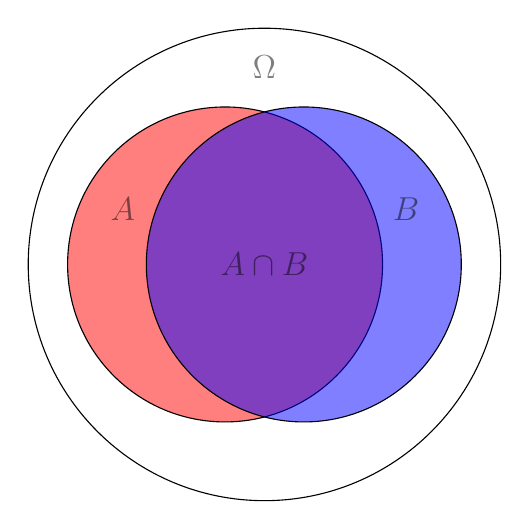
\begin{tikzpicture}
    \begin{scope}[shift={(3cm,-5cm)}, fill opacity=0.5]
        \draw[draw = black] (0,0) circle (3);
        \draw[fill=red, draw = black] (-0.5,0) circle (2);
        \draw[fill=blue, draw = black] (0.5,0) circle (2);
    \node at (0,2.5) (O) {\large\textbf{$\Omega$}};
    \node at (-1.8,0.7) (A) {\large\textbf{$A$}};
    \node at (1.8,0.7) (B) {\large\textbf{$B$}};
    \node at (0,0) (AetB) {\large\textbf{$A\cap B$}};
    \end{scope}
\end{tikzpicture}
\end{document}